%\documentclass[aps,prl,twocolumn,showpacs,superscriptaddress,groupedaddress]{revtex4}  % for review and submission
%\documentclass[aps,preprint,showpacs,superscriptaddress,groupedaddress]{revtex4}  % for double-spaced preprint
%\documentclass[aps,prl,floatfix,twocolumn,10pt]{revtex4-1}  % for review and submission
%\documentclass[aps,prl,preprint]{revtex4-1}  % for double-spaced preprint
\documentclass[aip,apl,amsmath,amssymb,floatfix,reprint,a4paper]{revtex4-1}

%% Packages
\usepackage{graphicx}  %figures
\usepackage{subfigure} %subfigures
\usepackage{amssymb}   %math
\usepackage{upgreek}   %non-italic greek letters
\usepackage[utf8]{inputenc} %Umlaute

%% hyphenation settings
\hyphenation{ALPGEN}
\hyphenation{EVTGEN}
\hyphenation{PYTHIA}

%% New commands
\newcommand{\unit}[1]{\ensuremath{\, \mathrm{#1}}}
\newcommand{\msub}[1]{\ensuremath{\textnormal{\begin{tiny}#1\end{tiny}}}}
\renewcommand{\d}[1]{\ensuremath{\operatorname{d}\!{#1}}}

%% ----------------------------------------------------------------------------------------------------------------
\begin{document}

\title{X-ray phase-contrast imaging at 100~keV}

\author{T.~Thüring}
  \affiliation{Paul Scherrer Institut, Villigen PSI, Switzerland}
  \affiliation{Institute for Biomedical Engineering, Swiss Federal Institute of Technology, Zurich, Switzerland}
\author{M.~Abis}
  \affiliation{Paul Scherrer Institut, Villigen PSI, Switzerland}
  \affiliation{Institute for Biomedical Engineering, Swiss Federal Institute of Technology, Zurich, Switzerland}
\author{Z.~Wang}
  \affiliation{Paul Scherrer Institut, Villigen PSI, Switzerland}
\author{C.~David}
  \affiliation{Paul Scherrer Institut, Villigen PSI, Switzerland}
\author{M.~Stampanoni}
  \affiliation{Paul Scherrer Institut, Villigen PSI, Switzerland}
  \affiliation{Institute for Biomedical Engineering, Swiss Federal Institute of Technology, Zurich, Switzerland}

\date{\today}


%% ----------------------------------------------------------------------------------------------------------------
\begin{abstract}
Phase contrast imaging with X-rays is an exciting field that reveals new insights into material properties by providing access to a complementary physical contrast mechanism. Phase sensitive imaging in the high energy range of hard X-rays, i.e. between $80$ and $150 \unit{keV}$ is still largely unexplored, as the current methods typically entail severe technical challenges. With a novel approach, we demonstrate phase contrast as well as dark-field contrast imaging on laboratory systems with low-brilliance X-ray sources in the entire diagnostic energy range. A phase-contrast technique at such high energies is of particularly high scientific and industrial interest as it would vastly expand the range of applications, for instance, by the examination of materials of high density or thickness. The approach includes a new technique for the grating manufacturing in Talbot-Lau interferometry. Firstly, the approach breaks the current limits of achievable grating aspect ratios, which has been a key issue for a long time in the past. Secondly, it solves the intrinsic reduction of the field of view which occurs for gratings with such high aspect ratios. Using an imaging arrangement based on a conventional X-ray tube, phase and dark-field-contrast imaging at $100 \unit{keV}$ is demonstrated for the first time. This achievement paves the road for the transfer of phase-contrast imaging into fields where high energies are required, such as medical CT, chip failure analysis or homeland security.
\end{abstract}

\maketitle

%%%%%%%%%%%%%%%%%%%%%%%%%%%%%%%%%%%%%%%%%%%%%%%%%%%%%%%%%%%%%%%%%%%%%%%%
% Body of manuscript
%%%%%%%%%%%%%%%%%%%%%%%%%%%%%%%%%%%%%%%%%%%%%%%%%%%%%%%%%%%%%%%%%%%%%%%%

X-ray radiography and computed tomography (CT) are nowadays standard imaging techniques in materials and life science for the non-destructive examination of samples or the diagnosis of diseases in patients. The underlying contrast mechanism relies on the different X-ray attenuation properties of two materials or tissue types. The dominant physical effects contributing to attenuation are the photo-electric effect and incoherent (Compton) scattering. The sum of their contributions determine the attenuation coefficient, which is a wavelenght dependent material parameter. Apart from attenuation, the wave nature of X-rays reveals another contrast mechanism, which is the phase shift. The physical interaction effect attributed to phase shifts is coherent (Rayleigh) scattering \cite{Als-Nielsen2011}.

Using the material parameter $n=1-\delta(\mathbf{r},\lambda) + i \beta(\mathbf{r},\lambda)$, known from X-ray wave optics as the complex index of refraction, the wavelenght dependent attenuation and phase shift properties of an object at the spatial coordinate $\mathbf{r}$ are fully described. The imaginary part $\beta(\mathbf{r},\lambda)$ is related to the attenuation per unit length (attenuation coefficient) by $\mu = 4 \pi \beta(\mathbf{r},\lambda) / \lambda$ and the total attenuation by an object of thickness $d$ can be described by the line integral $L_\mu = \int_0^d \mu(\mathbf{r},\lambda) \d l$. Similarly, the real part $\delta(\mathbf{r},\lambda)$ determines the phase shift per unit length by $\phi = 2 \pi \delta / \lambda$ and the total phase shift is $L_\phi = \int_0^d \phi(\mathbf{r}) \d l$.

While the attenuation line integral $L_\mu$ can be directly measured with an X-ray detector by measuring the reduction of the beam intensity $I$ ($L_\mu \propto \log(I)$), the measurement of the phase shift integral $L_\phi$ is more challenging as there is no such simple relation. However, phase sensitive imaging is a desirable modality, as it can provide an enhanced contrast-to-noise ratio (CNR) in images compared to attenuation for certain materials or in different tissue \cite{Pfeiffer2007a,McDonald2009}. Furthermore, the refractive index decrement $\delta$ provides direct access to the electron density \cite{Als-Nielsen2011} and in combination with attenuation, it further enables the determination of the effective atomic number of a material \cite{Qi2010}.

In the past, a lot of effort has been invested into the development of techniques which are sensitive to the phase shift. Since most of the available phase contrast techniques rely on interference and thus typically on optical hardware (e.g. crystals, gratings), they vary a lot in terms of sensitivity, practical applicability or achievable resolution. The vast majority of the methods, including crystal analyzer based \cite{Davis1995,Chapman1997} or interferometric \cite{Bonse1965,Momose1996} methods rely on X-ray beams of high spatial and temporal coherence, which is available only at synchrotron sources. Techniques which are compatible with an X-ray beam of low temporal coherence (broad bandwidth) are the in-line phase contrast method \cite{Snigirev1995,Wilkins1996,Cloetens1996} and Talbot interferometry \cite{Cloetens1997,David2002,Momose2003a}. Phase-contrast imaging using X-ray beams of low temporal \textit{and} spatial coherence (i.e. from low-brilliance X-ray sources) have been demonstrated with Talbot-Lau interferometry \cite{Pfeiffer2006} and coded apertures \cite{Munro2012}.

Phase-contrast imaging has so far been used in the lower diagnostic energy range, i.e. from $15$ up to $85 \unit{keV}$. Talbot interferometry has been demonstrated using a synchrotron source at $82 \unit{keV}$ \cite{Willner2013}. Also using a synchrotron source, phase-contrast imaging at $85 \unit{keV}$ has been reported. Using a low-brilliance X-ray tube, Talbot-Lau interferometry was applied at $60 \unit{keV}$ mean energy \cite{Donath2009}. Imaging applications which may benefit from phase contrast at higher energies are for instance medical imaging tasks; chest or abdominal radiography or CT require energies between $100$ and $150 \unit{keV}$. Other potential applications are homeland security or chip failure analysis, which require high energies for the visualization of materials of high density.

Here, we introduce a new method for phase-contrast imaging which is compatible with the entire diagnostic energy range of X-rays. Moreover, the method is fully compatible with compact imaging arrangements based on conventional X-ray tubes. The method is based on Talbot-Lau interferometry \cite{Pfeiffer2006} and employs a novel approach for the grating design and arrangement. Up to now, Talbot-Lau interferometry has been applied with a maximum design energy of $60 \unit{keV}$ \cite{Donath2009}. The challenge which limited the progress towards higher energies was mainly related to the manufacturing of gratings with high aspect ratios. The aspect ratio, given by
\begin{equation}
 \textnormal{AR} = \frac{2h}{p},
\end{equation}
where $p$ is the grating period and $h$ the grating structure height, is normally limited by the lithographic process, as grating structures tend to collapse or to deform (e.g. through capillary forces) if the aspect ratio is too high. For a given setup distance and for $p \propto 1/\sqrt{E}$ and $h \propto E^3$, it can be shown that $\textnormal{AR} \propto E^{7/2}$, where $E$ is the design energy of the system \cite{Momose2003a}. If at $E=25 \unit{keV}$ an aspect ratio for the absorption grating of around $\textnormal{AR}=30$ is necessary for a reasonable length of the experimental arrangement, it would have to be at least $128$ for $E=100 \unit{keV}$. Moreover, when using a polychromatic spectrum, photons above the design energy should also be efficiently attenuated by the gratings to guarantee their contribution to the signal, which requires even higher aspect ratios. Maximum achievable aspect ratios of current grating fabrication techniques \cite{David2007,Kenntner2010} are approximately around 60, whereas such high values are often even beyond the limit and come at the expense of a poor grating quality and performance.

Our approach is based on a new grating design which introduces the edge-on illumination of circularly aligned structures. Edge-on illumination, as opposed to face-on illumination, exploits the dimension along the grating lines to form a high aspect ratio of the structures in beam direction. The effective structure height of the grating is then determined by the grating dimension along the grating lines, which essentially allows arbitrarily high aspect ratios. FIG.~\ref{Fig:schematic} illustrates the edge-on illumination approach.
\begin{figure} [ht]
  \includegraphics[width = \linewidth]{figures/figure1.eps}
  \caption{Schematic of a grating interferometer for high X-ray energies in edge-on illumination mode. The aspect ratio is defined by the ratio of the travelling distance along the grating lines and the period and can be arbitrarily long. In order to avoid a reduction of the field of view, the grating structures are aligned on an arc.}
  \label{Fig:schematic}
\end{figure}

Increasing the effective aspect ratio of the gratings typically leads to a reduction of the field of view due to the change of the grating transmission function at high incident angles, which has also been identified by using a glancing angle of the gratings between zero and $90$ degrees \cite{Stutman2012a}. In order to overcome this problem with edge-on illuminated gratings, the grating lines are circularly aligned (i.e. on an arc) with a radius equal to the distance to the source.

The combination of edge-on illumination and circularly aligned structures enables phase-contrast imaging at arbitrary design energies and with a maximum field of view in horizontal direction ($x$ direction). These advantages come at the expense of a limited field of view in the vertical direction ($y$ direction), which is, depending on the X-ray detector, typically a few pixels. However, radiographic 2D imaging is possible in scanning mode, without increasing dose. Similarly, for tomographic images, the approach allows single slice CT or full 3D imaging in scanning mode.

Grating design and fabrication is non-standard and involves a complex mask design, as shown in FIG.~\ref{Fig:grating_mask}. Each grating resides on a silicon chip and has its specific structure length and curvature. For the present experiments, a symmetric interferometer with a grating period of $p = 2.8 \unit{\upmu m}$ for all gratings has been used. The design energy is $100 \unit{keV}$ and the beam splitter grating periodically shifts the phase by zero and $\pi$ at this energy \cite{David2002}. Using gold as the phase shifting material, this requires a structure length of $h_1 = 19.8 \unit{\upmu m}$. The analyzer grating is an absorption mask for sensing slight changes of the interference pattern generated by the beam splitter \cite{Momose2003a}. With a structure length of $h_2 = 800 \unit{\upmu m}$, this grating has an aspect ratio of $2h/p \approx 570$ and thus sufficiently attenuates X-rays up to energies of around $160 \unit{keV}$. Beam splitter- and analyzer grating are separated at the first fractional Talbot order \cite{Weitkamp2005}, resulting in an inter-grating distance of $158 \unit{mm}$. The source grating splits the relatively large focal spot ($\sim 1 \unit{mm}$) into an array of individually coherent, but mutually incoherent sources \cite{Pfeiffer2006}. It is also made of gold structures with a structure length of $h_0 = h_2 = 800 \unit{\upmu m}$.
\begin{figure} [ht]
  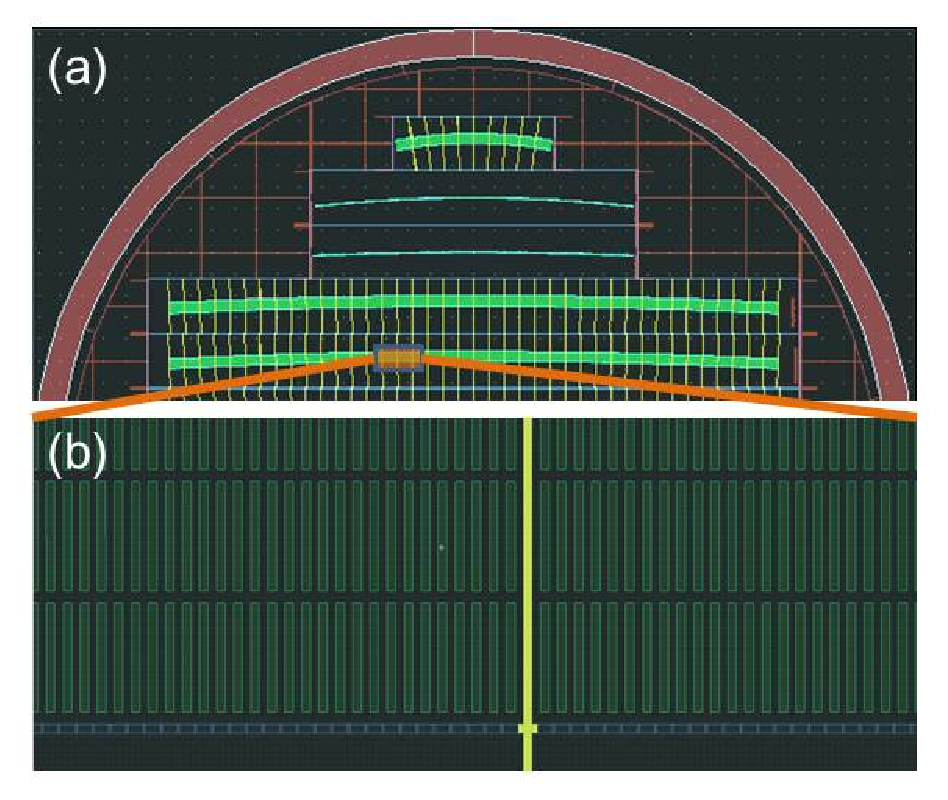
\includegraphics[width = \linewidth]{figures/grating_mask.eps}
  \caption{Grating design mask for the edge-on illumination approach. (a) Top part of the 4 inch wafer, showing five grating chips; one source grating, two beam splitter gratings and two analyzer gratings (from top to bottom). The gratings have different curvatures which are specific to the grating interferometer geometry. (b) Zoom into the grating structures, contain interrupting bridges used for stabilizing the grating structures in the lithographic process \cite{Kenntner2010}.}
  \label{Fig:grating_mask}
\end{figure}

Due to the high spectral acceptance \cite{Weitkamp2005,Thuering2013c} of the interferometer ($50 \unit{keV}$ to $>160 \unit{keV}$) and the high attenuation efficiencies of the source- and analyzer gratings ($>90\%$ up to $160 \unit{keV}$), the voltage of the X-ray source was set to the maximum of $160 \unit{kV}$. With a grating structure height of approx. $100 \unit{\upmu m}$, the field of view in the vertical direction is limited to one detector pixel row. In the horizontal direction, the field of view is limited by the grating size and the geometric magnification of the sample, yielding a maximum field of view of $30 \unit{mm}$. In addition to the standard components (source, camera, interferometer), two optical slits, one in front of the source grating, the other in front of the camera, were required for the collimation of the beam in the vertical direction. X-rays which are not travelling through all of the gratings do not contribute to the signal and are attenuated by the slits.

%Fig. 3 shows a radiographic image of a metal screw in all three contrast modes, acquired with the $100 \unit{keV}$ setup. The images were acquired in scanning mode, using a step size of $100 \unit{\upmu m}$. The number of phase steps was 24 and the exposure time was 15 seconds per step. Grating interferometry at such a high diagnostic energy allows to examine more dense materials such as metals in phase contrast mode. At lower energies, the phase shifts of such materials would be too large and wrap over multiple periods of the analyzer grating.

Fig.~\ref{Fig:img_chip} shows a radiographic scan of an electronic chip. Several resistors and an integrated circuit are located on different layers on the chip. The images were acquired in scanning mode, using a step size of $100 \unit{\upmu m}$ in $y$-direction. For a better comparison of the magnified phase and attenuation images, the attenuation image has been replaced with the differential attenuation image, which was obtained by digital differentiation. In the attenuation image, the soldering points of the integrated circuit are hardly visible underneath the resistors, while in the phase image, they can clearly be identified. This clearly implies the benefit of the differential nature of the phase-contrast image, which may be useful to identify flaws in multi-layered structures such as electronic chips.
\begin{figure} [ht]
  \includegraphics[width = \linewidth]{figures/img_chip_dabs.pdf}
  \caption{}
  \label{Fig:img_chip}
\end{figure}

Edge-on illuminated grating interferometry breaks the current limitations of phase-contrast imaging to the lower diagnostic energy range. Compact geometries  using conventional X-ray sources for design energies well above $100 \unit{keV}$ could be realized with the approach. This enables the examination of materials of higher density or thickness which would be intransparent at lower energies. Finally, the approach is not limited to X-ray imaging, but could easily be applied to other grating-based imaging modalities (e.g., with neutrons \cite{Grunzweig2008}) where high aspect ratios are required.

\section*{Methods}
Edge-on illuminated gratings were manufactured by Micro Works GmbH, Germany, using a LIGA process \cite{Kenntner2010}. Each grating resides on a $5 \times 60 \unit{mm^2}$ silicon chip and several grating chips are fabricated on a single 4 inch silicon wafer. The experimental arrangement for a design energy at 100 keV is a symmetric Talbot-Lau interferometer with a grating period of $p = 2.8 \unit{\upmu m}$ for all gratings. The distance from the source grating to the analyzer grating is $32 \unit{cm}$ and the source grating is positioned $23 \unit{cm}$ away from the source. The number of phase steps for one projection was 24 \cite{Weitkamp2005} and the exposure time for the images was 15 seconds per phase steps.

The X-ray source is a COMET MXR-160HP/11 X-ray tube with a maximum output voltage of $160 \unit{kV}$. In the experiment, it was set to the maximum voltage. The focal spot size is approximately $1 \unit{mm}$. The detector is a CCD camera from Finger Lakes Instruments. A cesium iodide (CsI:Ti) scintillator of $600 \unit{\upmu m}$ thickness converts the X-rays to visible light and is coupled with an optical lens projecting the image onto the CCD. The effective pixel size is $80 \unit{\upmu m}$. The widths of the collimating slits are $25 \unit{\upmu m}$ and $100 \unit{\upmu m}$, respectively.

In Fig.~\ref{Fig:img_chip}, image acquisition involved 24 phase steps \cite{Weitkamp2005} and an exposure time of 15 seconds per step.

\section*{Acknowledgements}
We thank Gordan Mikuljan from Paul Scherrer Institute, Switzerland, for his work on the mechanical design, Joachim Schulz and Marco Walter from Micro Works GmbH, Germany, for the competent support on grating design issues, Christian Kottler and Vincent Revol from Centre Suisse d'Electronique et de Microtechnique (CSEM), Switzerland for the fruitful discussions on the design of the system.


\bibliographystyle{apsrev4-1}
\bibliography{library}

\end{document}